\documentclass[]{article}
\usepackage{graphicx}
\usepackage{amsmath}

%opening
\title{Chapter 01: Foundations}
\author{Uday Manchanda}

\begin{document}

\maketitle

\begin{abstract}
\centering{Chapter 01 Notes in the book \textit{Applied Cryptography} by Bruce Schneier}
\end{abstract}

\section{1.1: Terminology}
\begin{itemize}
    \item Messages and Encryption
    \begin{itemize}
        \item Message is a plaintext
        \item Encrypted message is a ciphertext
        \item Cryptanalysis: breaking ciphertexts
        \item $E(M) = C$, the encryption function $E$ encrypts $M$ to obtain $C$
        \item $D(C) = M$, the decryption function $D$ decrypts $C$ to obtain $M$
        \item $D(E(M)) = M$
    \end{itemize}
    \item Authentication, Integrity, Nonrepudiation
    \begin{itemize}
        \item Authentication: receiver can ascertain its origin, intruder cannot masquerade as someone else
        \item Integrity: receiver should be able to verify that message has not been modified in transit
        \item Nonrepudiation: sender cannot later deny that he sent a message
    \end{itemize}
    \item Algorithms and Keys
    \begin{itemize}
        \item Cipher aka cryptographic algorithm is the mathematical function used for encryption and decryption
        \item Restricted algorithms, where the security of an algorithm is secret, are bad
        \item Modern crypto solves the problem with keys, where the range of possible values is the keyspace
        \item Both encrytion and decryption use the same key, although some algorithms use a different key for encryption and decryption
        \item Cryptosystem is an algorithm plus all possible plaintexts, ciphertexts, and keys
    \end{itemize}
    \item Symmetric Algorithms
    \begin{itemize}
        \item Encryption key can be calculated from the decryption key and vice-versa (usually the same)
        \item Sender and receiver must agree on a key
        \item Stream algorithm: operates on plaintext bit by bit
        \item Block algorithm: operates on plaintext in group of bits aka blocks
    \end{itemize}
    \item Public Key Algorithms
    \begin{itemize}
        \item Key for encryption is different than decryption key
        \item Encryption key (public key) is public, anyone can view it
        \item Anyone can use a public key to encrypt a message but only a specific person with the corresponding decryption key can decrypt it
        \item Decryption key is also known as the private key
    \end{itemize}
    \item Cryptanalysis
    \begin{itemize}
        \item Its about recovering the plaintext of a message without access to the key
        \item Losing a key through noncryptanalysis is a compromise
        \item Attempted cryptanalysis is an attack
        \item Seven types of cryptanalytic attacks
        \begin{itemize}
            \item \textbf{Ciphertext only attack}: the cryptanalyst has the ciphertext of several messages which have been encrypted with the same encryption algorithm. His job is to recover as many plaintexts as possible (or deduce the key used)
            \item \textbf{Known plaintext attack}: Cryptanalyst has ciphertext and plaintext of those messages. He has to deduce the key (or keys) used to encrypt the message
            \item \textbf{Chosen plaintext attack}: 0Cryptanalyst has access to the ciphertext and associated plaintext for several messages but also chooses the plaintext that gets encrypted. He/she can choose specific plaintext blocks to encrypt to reveal information about the key. 
            \item \textbf{Adaptive chosen plaintext attack}: Special case of a chosen plaintext attack. He can choose the plaintext that is encrypted, but also modify the choice based on results of previous encryption. 
            \item \textbf{Chosen ciphertext attack}: Cryptanalyst can choose different ciphertexts to be decrypted and has access to the decrypted plaintext. He must deduce the key.
            \item \textbf{Chosen key attack}: he has some knowledge about the relationship between different keys
            \item \textbf{Rubber hose cryptanalysis}: cryptanalyst threatens/blackmails someone until they give up the key
        \end{itemize}
        \item Known plaintext attacks and chosen plaintext attacks are relatively common
        \item Kerckhoff's assumption: secrecy must reside entirely in the key. Assume that the cryptanalyst has complete details of the cryptographic algorithm and implementation. 
        \item Always share the inner workings of your cryptgraphic implementations!
    \end{itemize}
    \item Security of algorithms
    \begin{itemize}
        \item Important that the value of the data remain less than the cost to break the security protecting it. 
        \item Categories of breaking algorithms
        \begin{itemize}
            \item Total break: cryptanalyst finds key
            \item Global deduction: cryptanalyst finds alternate algorithm that is equivalent to D without knowing K
            \item Instance deduction: cryptanalyst finds plaintext of an intercepted ciphertext
            \item information deduction: cryptanalyst gains some information about key or plaintext
        \end{itemize}
        \item If there is not enough information to recover plaintext from ciphertext, no matter how much ciphertext a cryptanalyst has, the algorithm is unconditionally secure
        \item Algorithm is computationally secure if it cannot be broken with current resources
        \item Can measure complexity of an attack by: data complexity, processing complexity, storage requirements
    \end{itemize}
\end{itemize}
\section{1.2: Steganography}
\begin{itemize}
    \item Steganography serves to hide secret messages in other messages, especially within pictures
\end{itemize}
\section{1.3: Substitution Ciphers and Transposition Ciphers}
\begin{itemize}
    \item Substitution Ciphers
    \begin{itemize}
        \item Where each character in the plaintext is substituted for another character in the ciphertext
        \item Four types of substitution ciphers
        \begin{itemize}
            \item Simple substitution cipher: each character of the plaintext is replaced with a corresponding character of ciphertext
            \item Homophonic substitution cipher: similar to previous except a single character of plaintext can map to several characters of ciphertext
            \item Polygram substitution cipher: blocks of characters are encrypted in groups
            \item Polyalphabetic substitution cipher: multiple sipmle substitution ciphers
        \end{itemize}
        \item Caesar cipher: each character in plaintext is replaced by character three to the right modulo 26
        \item ROT13: similar to casear except 13 instead of 3
    \end{itemize}
    \item Transposition Ciphers
    \begin{itemize}
        \item plaintext remains the same but order of characters is shuffled around
        \item Simple columnar transposition cipher: plaintext is written horizontally onto a piece of graph paper of fixed width 
        \item Frequency analysis of the characters is used
    \end{itemize}
\end{itemize}
\section{1.4: Simple XOR}
\begin{itemize}
    \item XOR = exclusive OR : $\oplus$
    \item If the digits are the same: 0, if different: 1
    \item $a \oplus a = 0$
    \item $a \oplus b \oplus b = a$
    \item Since XORing the same value twice restores the original, encryption and decryption use the same program
    \item $P \oplus K  = C$
    \item $C \oplus K  = P$
    \item How to break:
    \begin{itemize}
        \item Discover length of key by a procedure known as counting coincidences
        \item XOR ciphertext against shifted various number of bytes and count those bytes that are equivalent
        \item If the displacement is a multiple of the key length: $>$6\% of the bytes will be equal
        \item If not: $<$0.4\% will be equal
        \item This is known as index of coincidence
        \item Smallest displacement that indicates a multiple of the key length is the length of the key
        \item Shift ciphertext by that length and XOR with itself
        \item This removes the key and leaves with plaintext XORed with plaintext shifted the length of the key
        \item English has 1.3 bits of real information per byte
    \end{itemize}
\end{itemize}
\section{1.5: One Time Pads}
\begin{itemize}
    \item The perfect encryption scheme
    \item Large, nonrepeating set of truly random key letters
    \item Sender uses each key letter on the pad to encrypt exactly one plaintext character
    \item Add plaintext character plus one time key pad character and modulo 26
    \item As long as the attacker cannot get access to the one time pad, the scheme is perfectly secure
    \item Requires both the sender and receiver to agree on a pre-shared key
    \item Key letters have to be generated randomly, a psuedo random number does not work because it has nonrandom properties
    \item Cannot use the same pad again (hence, one time)
    \item Length of key pad and message must be the same
    \item Useful for short messages, nothing large
\end{itemize}
\section{1.6: Computer Algorithms}
\begin{itemize}
    \item Different types of cryptographic algorithms
    \begin{itemize}
        \item DES (Data Encryption Standard): symmetric algorithm, most popular one used, same key used for encryption and decryption
        \item RSA: most popular public key algorithm, used for encryption and digital signatures
        \item DSA (Digital Signature Algorithm): public key algorithm, used for digital signatures NOT encryption
    \end{itemize}
\end{itemize}
\section{1.7: Large Numbers}
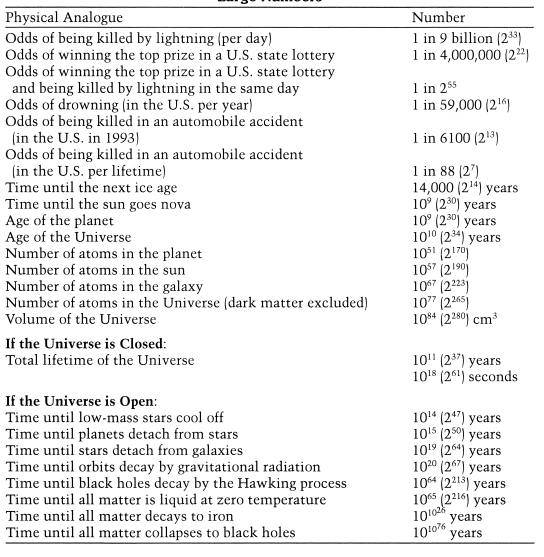
\includegraphics[width=0.75\textwidth]{largenumbers}
\end{document}